\chapter{Numerical Integration}\label{ch:integrals}


Like derivatives, integrals are also common mathematical tools used in physics.  Derivatives involve subtraction of similar values and suffer from bit-off errors.  Integration is essentially addition and thus numerical integration is a bit more robust than numerical derivative.  However, lots of addition incur significant round-off errors.  A good algorithm uses less addition without the expense of accuracy.  First, a simple method (rectangle rule) is used to demonstrate a basic idea of numerical integration.  Like forward finite difference method of numerical derivative, this method is not accurate enough for practical use.  However, a simple modification (trapezoidal rule), similar to mean finite difference method of numerical derivative, improves the accuracy.  More advanced methods (Simpson rule) will be introduced.

Improper integral needs special attention.   For example, when integral limits involve infinity like $\displaystyle\int_0^\infty f(x) \dd{x}$,  most numerical integration methods require infinitely many addition, which cannot be done.  Another example is the case where integrand has integrable singularities like $\displaystyle\frac{1}{\sqrt{x}}$.  Since we cannot evaluate the function value at $x=0$, the common numerical methods fail.  There is no systematic resolution to these problems.  We need to deal with them on case-by-case basis.  Several common practices will be introduced in this chapter.
In addition, a magic method called Gaussian quadrature, which gives rather accurate results for certain types of integrals just by computing several points, will be discussed.

\section{Rectangular rule}\label{sec:rectangular-rule}
	
We want to integrate a function $f(x)$ from $a$ to $b$.
Similarly to the numerical derivative problems, there are two different cases.  In one case, a closed form expression of the function is known and we can evaluate the function value at any point of $x \in [a,b]$.  In the other case, the function values are given as a finite sequence $f_n = f(x_n), n=0, \cdots, N$ and the analytical expression of the function is unknown. In this section, we focus on the former case and the latter case will be discussed in a later chapter.

\begin{figure}
	\centering
	\begin{subfigure}{0.45\textwidth}
		\centering
		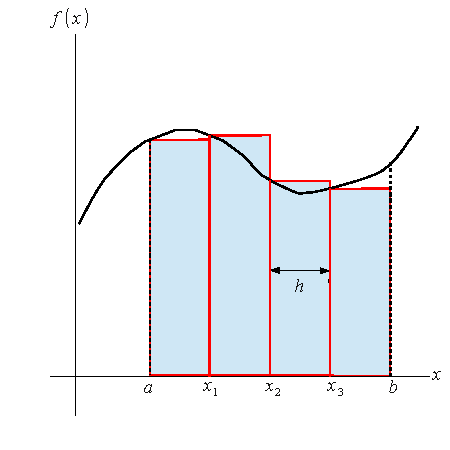
\includegraphics[width=3in]{03.integrals/int-rectangle.pdf}
		\caption{Forward rectangular method. The large errors are clearly visible.}
		\label{fig:int-rectangle}
	\end{subfigure}
	\begin{subfigure}{0.45\textwidth}
		\centering 
		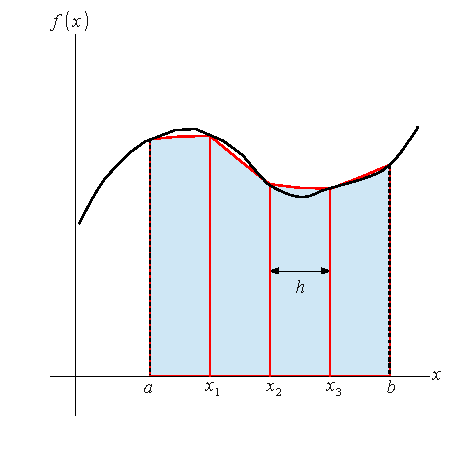
\includegraphics[width=3in]{03.integrals/int-trapezoid.pdf}
		\caption{Trapezoidal method. The errors are much smaller than those in the rectangular method.}
		\label{fig:int-trapezoid}
	\end{subfigure}
	\caption{Illustration of simple numerical integration methods}
\end{figure}


We begin with the Rieman's definition of integral:
\begin{equation}
\int_{a}^{b} f(x) \dd{x} = \lim_{N \rightarrow \infty} \sum_{n=0}^{N-1} f(x_n)\, h  = \lim_{N \rightarrow \infty} \sum_{n=1}^{N} f(x_n)\, h
\end{equation}
where $h =(b-a)/N$ and $x_n=a + n\, h$.   Note that $h$ depends on $N$.  Numerical methods do not understand this kind of limit since it ends up with $\infty \times 0$.  Beside, summing infinitely many terms costs infinite CPU time.  We hope that sufficiently large $N$ (i.e., sufficiently small $h>0$) gives a value close to the exact integral. This is the rectangular rule:
\begin{subequations}\label{eq:rectangular-rule}
\begin{equation}\label{eq:fwd-rectangle}
\int_{a}^{b} f(x) \dd{x} \approx \hat{I}_\text{F} f(x) \equiv \sum_{n=0}^{N-1} f(x_n)\, h 
\end{equation}
\begin{equation}\label{eq:bwd-rectangle}
\int_{a}^{b} f(x) \dd{x} \approx \hat{I}_\text{B} f(x) \equiv\sum_{n=1}^{N} f(x_n)\, h
\end{equation}
\end{subequations}
where $\hat{I}_\textbf{F}$ and $\hat{I}_\textbf{B}$ are forward and backward rectangular rule operator, respectively.

\begin{myalgobox}
    \Algorithm{Integration by the forward rectangular rule}\label{algo:fwd-rectangle}
    
    \medskip
    The following steps evaluate Eq. \ref{eq:fwd-rectangle}.
    
    \medskip
    \begin{enumerate}
        \item Set the step length: $h=\displaystyle\frac{b-a}{N}$
        \item Set $s=0.0$ where $s$ should be double (float64).
        \item Repeat steps 4-6 for $n=0$ to $n=N-1$:
        \item $x=a+n*h$.
        \item $s=s+f(x)$.  [where $f(x)$ can be inline function or funtion subprogram.]
        \item Go back to step 4 and repeat with new $n$.
        \item The integral is given by $s*h$.
    \end{enumerate}

\bigskip
Steps 3-6 can be simplified using \texttt{linspace} and \texttt{sum} functions. See sample codes.
\end{myalgobox}


The forward rectangular rule is illustrated in Fig \ref{fig:int-rectangle}. The integral [the area below the curve $f(x)$] is approximated by the sum of many small rectangles.
However, the large errors are clearly seen in the illustration where the slope of curve is steep.

To investigate the error in the rectangular rule, we consider the small integral interval from $x_{n}$ to $x_{n+1}=x_n+h$.  Expanding the integral with respect to $h$ (See Appendix \ref{ap:int_expand}),  the integral is expressed as power series of $h$:
\begin{equation}\label{eq:int+expand}
\int_{x_{n}}^{x_{n}+h} f(x) \dd{x} = f(x_n) h + f'(x_n) \frac{h^2}{2} + f''(x_n) \frac{h^3}{3!} + + f^{(3)}(x_n) \frac{h^4}{4!} + \order{h^5}.
\end{equation}
Then, the whole integral in the forward scheme is expressed as
\begin{equation}
\int_a^b f(x) \dd{x} = \sum_{n=0}^{N-1} \int_{x_{n}}^{x_{n}+h} f(x) \dd{x} =  \sum_{n=0}^{N-1} \left [f(x_n) h + f'(x_n) \frac{h^2}{2} + \order{h^3} \right ]
\end{equation}
By neglecting $h^2$ and higher orders, we obtain the rectangular rule.
Therefore, the error of the rectangular rule is the order of $h^2$ per segment.  Since there are $N$ segments, the total error is
order of $h^2 N = (b-a) h$.  Hence, the total error is the order of $h$.  You might think that if a very small value of $h$ is used the error is negligible. Unfortunately, the round-off error gets too large when $N$ is too large (See Example 1.8). In practice, this method is rarely used.

\section{Trapezoidal rule}


It is better to approximate the area using trapezoids as shown in Fig \ref{fig:int-trapezoid}.
\begin{eqnarray}\label{eq:trapezoidal rule}
\int_a^b f(x)\, \md x &\approx& \hat{I}_{T} f(x) \equiv \sum_{n=0}^{N-1}\, \frac{f(x_{n+1})+f(x_{n})}{2}\, h \\
&=& \fbox{$\displaystyle\frac{h}{2} \left [ f(a) + f(b) \right ] + \sum_{n=1}^{N-1} f(x_n) h $}
\end{eqnarray}
The trapezoidal rule is equivalent to the mean of the forward and backward rectangular rules, i.e., $\hat{I}_\text{T} f(x) = \frac{1}{2} \left [ \hat{I}_\text{F} + \hat{I}_\text{B} \right ]f(x)$.  Note also that the difference between the trapezoidal rule and the rectangular rule is only how the end points $f(a)$ and $f(b)$ are treated:
\begin{equation}
\hat{I}_\text{T} f(x) = \hat{I}_\text{F} f(x)+\frac{h}{2} \left [ f(a) - f(b) \right ] = \hat{I}_\text{B} f(x) - \frac{h}{2} \left [ f(a) - f(b) \right ]
\end{equation}
Nevertheless, this simple modification improve the accuracy significantly.  

Let us find the order of error by substituting the forward finite difference method, $f'(x_n) = \displaystyle\frac{f(x_n+h)-f(x_n)}{h}+\order{h}$ into Eq. (\ref{eq:int+expand}):
\begin{equation}\label{eq:error_trapezoid} 
\int_{x_{n}}^{x_{n+h}} f(x) \dd{x} = f(x_n) h + f'(x_n)\frac{h^2}{2} + \order{h^3} = \frac{f(x_n)+f(x_{n+1})}{2} h + \order{h^3}.
\end{equation}
If $h^3$ and higher orders is ignored, we obtain the trapezoid rule.  Hence, the trapezoidal rule is locally accurate up to $h^2$, better than the rectangular rule.  The total error is the order of $h^3 N =(b-a) h^2$.  The trapezoidal method is commonly used due to its simplicity and reasonable accuracy. Interestingly, if the function vanishes at the integral limits, $f(a)=f(b)=0$, then the rectangular rule produces exactly the same result as the trapezoidal rule.

\begin{myalgobox}
    \Algorithm{Integration by the trapezoidal rule}\label{algo:trapezoidal rule}
    
    \medskip
    The following steps evaluate Eq. \ref{eq:trapezoidal rule}.
    
    \medskip
    \begin{enumerate}
        \item Set the step length: $h=\displaystyle\frac{b-a}{N}$
        \item Set $s=0.5*(f(a)+f(b))$ where $s$ should be double (float64).
        \item Repeat steps 4-6 for $n=1$ to $n=N-1$:
        \item $x=a+n*h$.
        \item $s=s+f(x)$.  [where $f(x)$ can be inline function or funtion subprogram.]
        \item Go back to step 4 and repeat with new $n$.
        \item The integral is given by $s*h$.
    \end{enumerate}

\bigskip
    Steps 3-6 can be simplified using \texttt{linspace} and \texttt{sum} functions. See sample codes.
\end{myalgobox}



\section{Simpson method}

There is an even better method.
In Eq. (\ref{eq:int+expand}) the rectangular method ignored $f'(x)$ and all higher order derivatives.  That means the function $f(x)$ is approximated by piece-wise constant functions (no slope). Note that you need only one function value $f(x_n)$ to calculate the area of the rectangle.  To increase the accuracy, the slope of the function, $f'(x)$ in Eq. (\ref{eq:int+expand}), is taken into account in the trapezoidal method. That means two function values $f(x_n)$ and $f(x_{n-1})$ are needed to compute the area of the individual segment.  Natural extension to this line of approximation is to take into account the curvature or $f''(x)$.  Noting that the evaluation of $f''(x)$ requires three data points, we utilize the another expansion similar to Eq. (\ref{eq:int+expand}),
\begin{equation}\label{eq:int-expand}
\int_{x_{n}}^{x_{n}-h} f(x) \dd{x} = -f(x_n) h + f'(x_n) \frac{h^2}{2} - f''(x_n) \frac{h^3}{3!} + +f^{(3)}(x_n) \frac{h^4}{4!} + \order{h^5}
\end{equation}
Using the expansions (\ref{eq:int+expand}) and (\ref{eq:int-expand}), we find the integral from $x_{n-1}$ to $x_{n+1}$ as
\begin{equation}\label{eq:int+-expand}
\int_{x_n-h}^{x_n+h} f(x) \dd{x} = 2 f'(x_n) h + 2 f''(x_n) \frac{h^3}{3!} + \order{h^5}
\end{equation}
Note that the fourth order term is canceled out, which makes this approximation accurate.
Substituting the finite difference formula of the second order derivative [Eq \eqref{eq:diff2-s3} in Chapter \ref{ch:derivatives}] into Eq. \eqref{eq:int+-expand}, we find the integral 
\begin{equation}
\int_{x_{n-1}}^{x_{n+1}} f(x) \dd{x} = \left [ \frac{1}{3} f(x_{n-1})+ \frac{4}{3} f(x_n) + \frac{1}{3} f(x_{n+1}) \right ] h + \order{h^5},
\end{equation}
which leads to local error at the order of $h^5$.
Repeating this formular, we obtain the Simpson rule
\begin{equation}\label{eq:simpson_rule}
\int_{a}^{b} f(x) \dd{x} \approx \hat{I}_\text{S} \equiv 
\fbox{$\displaystyle\sum_{j=0}^{N/2-1} \left [ f(x_{2j})+4 f(x_{2j+1})+f(x_{2j+2}) \right ] \frac{h}{3}$} + \order{h^4}
\end{equation}
The error of the Simpson rule is the order of $h^5$ per segment and thus $h^4$ for the whole integral which is two orders of magnitude better than that of the trapezoidal rule.

\begin{myalgobox}
    \Algorithm{Integration by the Simpson rule}\label{algo:simpson rule}
    
    \medskip
    The following steps evaluate Eq. \ref{eq:simpson_rule}.
    
    The number of points $N$ should be even.
    \medskip
    \begin{enumerate}
        \item Set the step length: $h=\displaystyle\frac{b-a}{N}$
        \item Set $s=-f(a)-f(b)$ where $s$ should be double (float64).
        \item Repeat steps 4-6 for $j=0$ to $j=N/2-1$:
        \item $x=a+2*j*h$.
        \item $s=s+2.0*f(x)+4.0*f(x+h)$. 
        \item Go back to step 4 and repeat with new $j$.
        \item The integral is given by $s*h/3.0$.
    \end{enumerate}

\bigskip
Steps 3-6 can be simplified using \texttt{linspace} and \texttt{sum} functions. See sample codes.
\end{myalgobox}


\begin{figure}[b]
	\centerline{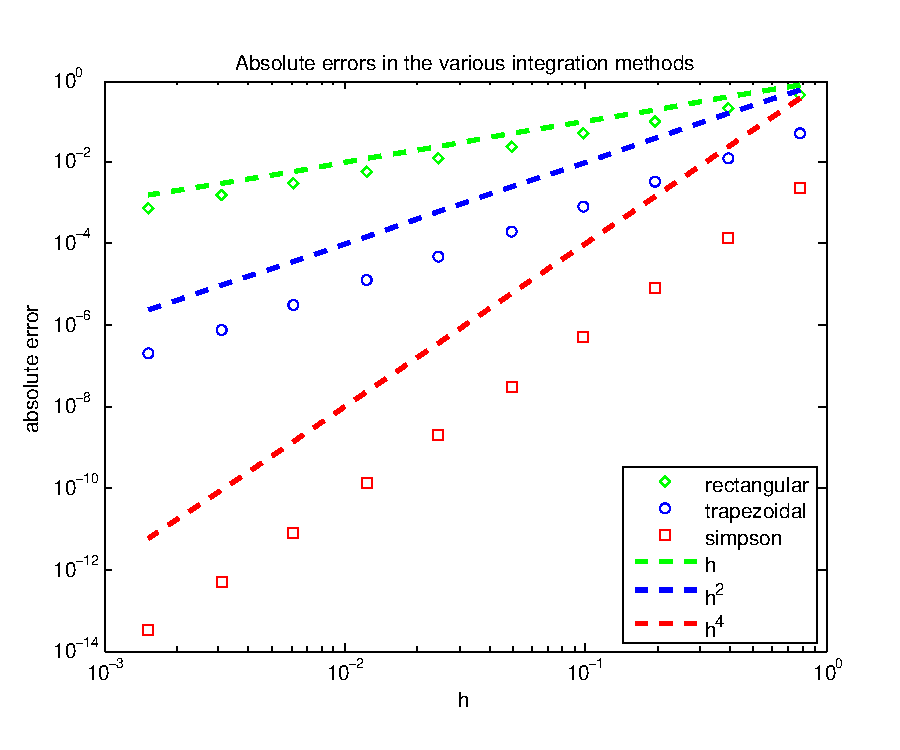
\includegraphics[width=3.5in]{03.integrals/integral-plot.pdf}}
	\caption{Output of Example \ref{ex:integrals}.}
	\label{fig:integrals}
\end{figure}

\bigskip
\begin{example}[Errors in various numerical integration methods]\label{ex:integrals}

Let's integrate $\sin(x)$ from $x=0$ to $x=\pi/2$.  The exact answer is
$\cos(0)-\cos(\pi/2)=1$. Program \ref{matlab:integrals} computes the integral  using the rectangular, trapezoidal, and Simpson rules.
The error of each rule is plotted in Fig. \ref{fig:integrals}. As $h$ decreases, the error also decreases with all methods.  The Simpson rule has small errors even at $h=0.1$.
\end{example}

\vspace{18px}
\noindent
\exercise
Numerically integrate $f(x)=\displaystyle\frac{\sin(x)}{1+x^2}$ from $x=0$ to $x=\pi$.

Analytical solution by Mathematica is
\begin{eqnarray}\label{eq:trig_int}
 \int_0^\pi \frac{\sin(x)}{1+x^2} \dd{x} &=&  \frac{e}{4} \left[-2 \text{Ci}(i)+\text{Ci}(i-\pi )+\text{Ci}(i+\pi )+2 \text{Shi}(1)+i \text{Si}(i-\pi )+i \text{Si}(i+\pi )\right ] \nonumber \\ 
	&&+\frac{1}{4e} \left [2 \text{Ci}(i)-\text{Ci}(i-\pi )-\text{Ci}(i+\pi )+2 \text{Shi}(1)+i \text{Si}(i-\pi )+i \text{Si}(i+\pi ) \right ]
\end{eqnarray}
where Ci, Si, and Shi are trigonometric integral functions.
The answer should be real but Eq. \ref{eq:trig_int} contains imaginary unit.  It is not obvious that the imaginary parts are canceled out. This expression is too complicated to see the answer.  Analytical solution is not always useful.  Furthermore, these trigonometric integrals must be numerically evaluated.  So, why don't we evaluate the original integral numerically from the beginning? 

\subsection{Adaptive quadrature}

As demonstrated above, the accuracy of numerical integration depends on the choice of the grid interval $h$.  In practice, finding an appropriate value for $h$ is  tedious. Especially when the integrand $f(x)$ changes rapidly in some region and smooth in other region (\textit{stiff} function), a small value of $h$ is necessary only for the rapidly changing region.    If a constant $h$ is used for the whole region, we may be wasting computer time.   Technically speaking, it is possible to use different $h$ but it is quite cumbersome to do it manually.  Therefore, we ask computer to find the best value of $h$ at each point, which is known as adaptive grid method.

The basic idea is simple. First, we integrate the function using three grid points $x_1$ and $x_2$ with interval $h^{(0)}$.  Here the index $^{(0)}$ indicates the depth of adaptivity.  Let us call the result of the integration $I^{(0)}$.  Then, we integrate the function between $x_1$ and $x_2$ again using the interval $h^{(1)}=h^{(0)}/2$ and obtain a new result $I^{(1)}$.  If the difference between $I^{(0)}$ and $I^{(1)}$ is smaller than a specified tolerance, we accept $I^{(1)}$ as accurate result and move on to the next segment.  If not, we reduce the interval again as $h^{(2)}=h^{(1)}/2$.  We repeat this until the error becomes small enough.



\begin{example}[Adaptive Quadrature]
Let us numerically calculate the integral
\[
I=\int_0^5 (4x-x^2) e^{-2x} \dd{x}
\]
whose exact value is $\displaystyle\frac{3}{4} + \frac{17}{4} e^{-10}\sim 0.75019294970149056062$.  The integrand rises very rapidly and decreases to zero slowly.  We will evaluate it using the adaptive quadrature.
MATLAB has built-in function \texttt{integral(func,xmin,xmax)} which uses adaptive quadrature with a default error tolerance (Absolute error = $10^{-10}$ and relative error = $10^{-6}$).  Instead of writing our own code, we will use it this time.
\begin{mybox}
\small
\begin{verbatim}
>> fprintf('%24.16e\n',integral(@(x) (4*x-x.^2).*exp(-2*x),0,5))
  7.5019294970149075e-01
\end{verbatim}
\normalsize
\end{mybox}

\end{example}

\noindent
\section{Improper Integrals}

When the integral limit involves infinity, the numerical methods we discussed above won't work since the number of grid points become infinity.  If the integrand is singular at a point within the integral limit, again the regular method fails.  We need special methods.  In the following, we discuss some of simple ways to avoid such difficulty.

\noindent
\subsection{Improper Integrals: $\infty$ in Limits}

If the upper limit is $\infty$ or the lower limit is $-\infty$, for example, $\displaystyle\int_0^\infty f(x)\, \md x$, all the methods we discussed so far cannot be used. One way to overcome this problem is to split the integral to two parts
\begin{equation}
\int_0^\infty f(x) \dd{x} = \int_0^a f(x) \dd{x} + \int_a^\infty f(x) \dd{x}
\end{equation}
where $a$ is a positive constant.
The first term in the right hand side can be integrated by the trapezoidal or simpson rule. The second term needs to be transformed to a numerically computable form by introducing a new variable $t=\displaystyle\frac{1}{x}$. Then, the integral we need to compute is
\begin{equation}
\int_a^\infty f(x) \dd{x} = \int_0^{1/a} \frac{1}{t^2}\, f\left (\frac{1}{t} \right ) \dd{t}
\end{equation}
The integral in the right hand side can be integrated by a standard method. However, the new form is not necessarily trouble free since the integrand is not defined at the lower bound (divided-by-zero error). If we can evaluate $\lim_{t \rightarrow 0} 1/t^2 f(1/t)$ analytically by hand, then standard methods such as the Simpson method works. 

 The following types of improper integral:
\begin{eqnarray}
\int_0^\infty \me^{-x} f(x) \dd{x} &\qquad& \text{Use Gauss-Laguerre quadrature.} \\
\int_{-\infty}^{\infty} \me^{-x^2} f(x) \dd{x} &\qquad& \text{Use Gauss-Hermite quadrature.}
\end{eqnarray}
can be evaluated by the Gaussian quadrature which we will discuss in Section \ref{sec:Gaussian_Quadrature}.

\noindent
\subsection{Improper Integrals II:  Integrable Singularities}

If the integrand has integrable singularities such as $\displaystyle\frac{1}{\sqrt{x}}$ within the integral limits, the standard methods fail. Such improper integrals are ubiquitous in physics.  A common method is to isolate the singularity and integrate it analytically.  Then, we integrate the remaining part by a numerical method.  



\bigskip
\begin{example}[Removal of Integral Singularity]
\label{ex:improper_int}
\begin{figure}[t]
\centerline{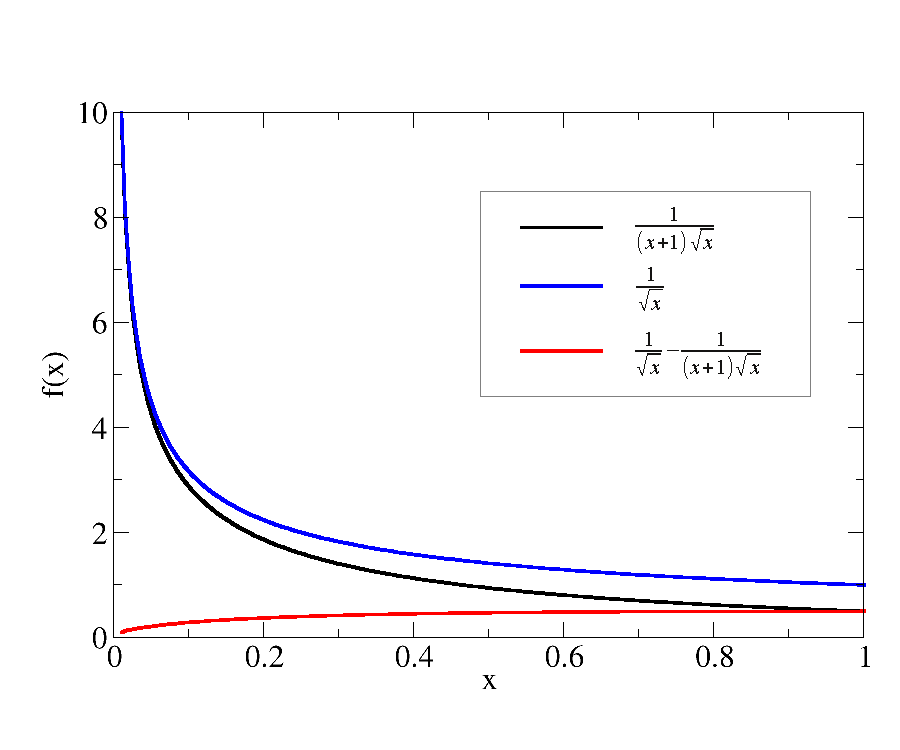
\includegraphics[width=3.5in]{03.integrals/improper_int_example.pdf}}
\caption{Due to the divergence at $x=0$, it is difficult integrate the original function (black line).  The blue line has the same singularity at $x=0$ but can be analytically integrate.  The difference (red line) does not have a singularity and hence common numerical integration works fine.}
\label{fig:improper_int}
\end{figure}

Consider an improper integral
\begin{equation}
\int_0^a \frac{1}{(1+x)\sqrt{x}} \dd{x} = \pi - 2 \arctan \left ( \frac{1}{\sqrt{a}} \right )
\label{eq:improper_int}
\end{equation}
where $a$ is a positive constant. This integral is finite despite that the integrand diverges at $x=0$. For $x=\epsilon\ll 1$, the integrand can be expanded as
\begin{equation}
\frac{1}{(1+\epsilon)\sqrt{\epsilon}} \sim \frac{1-\epsilon}{\sqrt{\epsilon}} \sim \frac{1}{\sqrt{\epsilon}}
\end{equation}
Hence, the singularity is $\displaystyle\frac{1}{\sqrt{\epsilon}}$. We split the integral in two parts as follows:
\begin{eqnarray}
\int_0^a \frac{1}{(1+x)\sqrt{x}}\, \md x &=& \int_0^a \frac{1}{\sqrt{x}} \dd{x} + \int_0^a \left [ \frac{1}{(1+x)\sqrt{x}}
 - \frac{1}{\sqrt{x}} \right ] \dd{x} \nonumber \\
 &=& 2 \sqrt{a} - \int_0^a \frac{\sqrt{x}}{1+x} \dd{x} 
\end{eqnarray}
The last integral is not improper and thus can be integrated by a standard method. Indeed, Fig. \ref{fig:improper_int} shows that the new integrand has no singularity at $x=0$ and the curve is very smooth.  In addition the integral of this function is small compared with the integral of the singular part. Hence, numerical error is reduced.

Program \ref{matlab:improper_int} computes integral (\ref{eq:improper_int}).  The proper part of the integral is done with the trapezoidal rule.  The result is compared with the analytic solution.  Using $a=1$, $h=0.01$, the program produces the output

\begin{mybox}
\small
\begin{verbatim}
Numerical = 1.571003957326e+00
    Exact = 1.570796326795e+00
\end{verbatim}
\normalsize
\end{mybox}

\bigskip\noindent
Only the first three figures are correct, but which is acceptable in most cases.
\end{example}

\noindent
\section{Gaussian Quadrature}\label{sec:Gaussian_Quadrature}

The Gaussian quadrature magically evaluates improper integrals utilizing the properties of orthogonal polynomials such as Legendre and Laguerre polynomials.  Despite the integral limit is infinity, you need to evaluate the integrand only at several points.  The theoretical justification of the Gaussian quadrature needs knowledge of special functions. Here we show only the formulas. See Appendix \ref{app:gauss-quad} for the theory behind the Gaussian quadrature.  

\begin{itemize}
\item Gaussian-Laguerre Quadrature
\begin{equation}\label{eq:gauss-laguerre}
\int_0^\infty f(x) \me^{-x} \dd{x} = \sum_{i=1}^{N} w_i f(x_i)
\end{equation}
where weight $w_i$ and abscissa $x_i$ are given in Table \ref{tab:Gaussian-Laguerre}.

\item Gaussian-Hermite Quadrature
\begin{equation}\label{gauss-hermite}
\int_{-\infty}^\infty f(x)\, \me^{-x^2} \dd{x} = \sum_{i=1}^{N} w_i f(x_i)
\end{equation}
where weight $w_i$ and abscissa $x_i$ are given in Table \ref{tab:Gaussian-Hermite}. 

\item Gaussian-Legendre Quadrature
\begin{equation}\label{gauss-legendre}
\int_{-1}^1 f(x) \, \dd{x} = \sum_{i=1}^{N} w_i f(x_i)
\end{equation}
where weight $w_i$ and abscissa $x_i$ are given in Table \ref{tab:Gaussian-Legendre}. 

\end{itemize}
These formula work well if $f(x)$ behaves like a polynomial as $x \rightarrow \infty$. It fails if $f(x)$ behaves like an exponential function.  

\begin{example}[Magical Gaussian Quadrature]
\label{ex:blackbody}
The energy density of blackbody radiation at temperature $T$ is given by
\begin{equation}
u(T) = \frac{8 \pi (k T)^4}{(h c)^3} J
\end{equation}
where $h$, $c$, and $k$ are Plank constant\cite{Griffiths}, speed of light, and Boltzmann constant\cite{Blundell}.
The factor $J$ is a dimensionless constant determined by integral:
\begin{equation}
J = \int_0^\infty \frac{x^3}{\me^x  - 1} \dd{x} = \frac{\pi^4}{15}
\end{equation}
Let us try to integrate it numerically and compare the result with the exact value.  Since the integral bounds are 0 and $\infty$, we use the Gaussian-Laguerre quadrature.
To use the Gaussian-Laguerre quadrature, the integrand must have $\me^{-x}$. We can always create $\me^{-x}$ by multiplying $\me^{x}\, \me^{-x}$ to the integrand. Now we have the desired exponential function $\me^{-x}$, but as a penalty another exponential function $\me^{x}$ is introduced in the integrand which is now $f(x)=\displaystyle\frac{x^3 \me^{x}}{\me^{x}-1}$.   We need to make it sure that the extra $\me^x$ does not cause a problem.  Since $f(x) \rightarrow x^3$ as $x \rightarrow \infty$, $f(x)$ behaves like a polynomial and thus the Gaussian quadrature is expected to give a good result.  Program \ref{matlab:gauss-lagurre} calculate $J$ using the Gauss-Laguerre quadrature.  The output is 

\begin{mybox}
\small
\begin{verbatim}
8 points Gaussian Laguerre Quadrature
Exact= 6.493939402267e+00
Gauss= 6.493935665353e+00 
Error= 3.736914144348e-06
\end{verbatim}
\normalsize
\end{mybox}

\medskip
\noindent
Despite that we evaluated the integrand only at 8 points, the agreement with the exact value is remarkable.

\end{example}

\noindent
\section{Applications in Physics}


\bigskip
\subsection{Period of Classical Oscillation I.}\label{sec:oscillation1}

\begin{figure}
\centerline{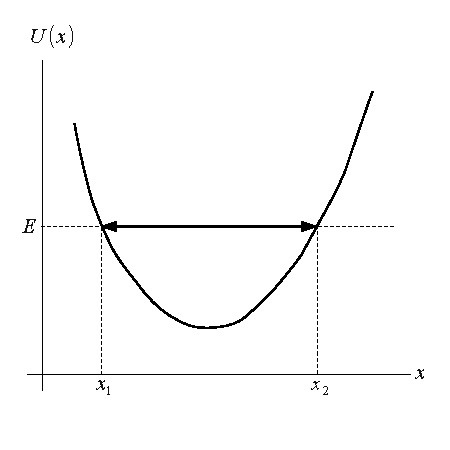
\includegraphics[width=2.5in]{03.integrals/oscillation.pdf}}
\caption{Classical Oscillation}\label{fig:oscillation}
\end{figure}

\medskip
\noindent
A classical particle with energy $E$ is confined in a potential $U(x)$. (See Fig \ref{fig:oscillation}.)  The particle oscillates between turning points $x_1$ and $x_2$.  The period of oscillation\cite{Taylor2005} is given by
%
\begin{equation}\label{eq:oscillation-period}
T=2 \int_{x_1}^{x_2} \frac{1}{v(x)} \dd{x}
\end{equation}
%
where the speed of the particle at $x$ is given by
%
\begin{equation}\label{eq:vx}
v(x) = \sqrt{\frac{2(E-U(x))}{m}}
\end{equation}
The integral bounds are determined by solving $v(x)=0$, which requires numerical root finding discussed in next Chapter.

The integral in Eq. (\ref{eq:oscillation-period}) is improper since $v(x_1)=v(x_2)=0$.  We need to remove the integral singularities. First we expand the potential around the turning points:
%
\begin{equation}
U(x) = U(x_i) + U'(x_i) (x-x_i) + o(x^2)=E + U'(x_i) (x-x_i) + o(x^2), \qquad i=1,2
\end{equation}
%
If the potential is approximated by $U_i(x) = E+U'(x_i)(x-x_i)$, the speed becomes 
%
\begin{equation}
v_i(x) = \sqrt{\frac{-2U'(x_i)(x-x_i)}{m}}
\end{equation}
%
Note that this approximated speed approaches to the correct speed as $x \rightarrow x_i$.  Utilizing it, we remove the singularities as follows.
%
\begin{eqnarray}
\int_{x_1}^{x_2} \frac{1}{v(x)} \dd{x} &=& \int_{x_1}^{x_0} \left [\frac{1}{v(x)}-\frac{1}{v_1(x)}\right ] \dd{x} 
+ \int_{x_1}^{x_0} \frac{1}{v_1(x)} \dd{x} \\
&+& \int_{x_0}^{x_2} \left [\frac{1}{v(x)}-\frac{1}{v_2(x)}\right ] \dd{x} + \int_{x_0}^{x_2} \frac{1}{v_2(x)} \dd{x}\\
\end{eqnarray}
%
where $x_0$ is any point between $x_1$ and $x_2$.  A good choice would be a point where the potential is minimum.  The integrands inside the square brackets have no singularity and thus can be integrated using a common numerical method. The remaining integral can be easily evaluated analytically:
%
\begin{eqnarray}
\int_{x_1}^{x_0} \frac{1}{v_1(x)} \dd{x} &=& \sqrt{\frac{m}{-2 U'(x_1)}} \int_{x_1}^{x_0} \frac{1}{\sqrt{x-x_1}} \dd{x}
=\sqrt{\frac{2 m x_0}{|U'(x_1)|}} \\
\int_{x_0}^{x_2} \frac{1}{v_2(x)} \dd{x} &=& \sqrt{\frac{m}{2 U'(x_2)}} \int_{x_0}^{x_2} \frac{1}{\sqrt{x_2-x}} \dd{x}\, .
=\sqrt{\frac{2 m x_0}{|U'(x_2)|}}
\end{eqnarray}
%


\subsection{Scattering by Yukawa Potential: Part 1}
\label{sec:scattering1}

\begin{figure}
\centerline{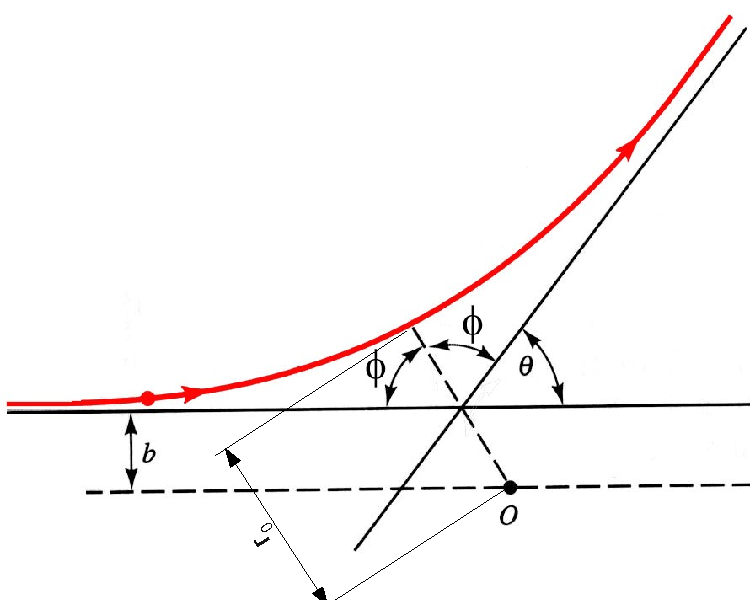
\includegraphics[width=3.0in]{03.integrals/scattering-diagram.pdf}}
\caption{Geometry of scattering in relative coordinate.}
\label{fig:scattering}
\end{figure}

\begin{figure}[bt]
\centerline{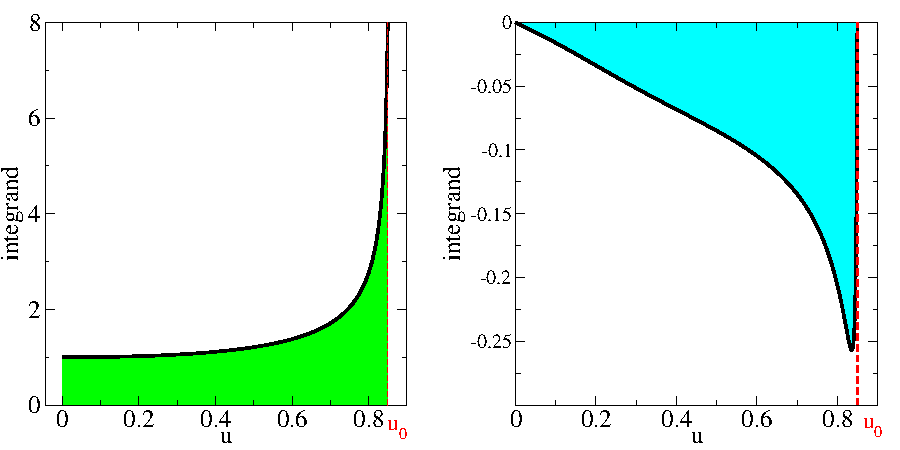
\includegraphics[width=5.0in]{03.integrals/scattering-integrand.pdf}}
\caption{
The left panel shows the original integrand.  The green area need to be
numerically integrated. The right panel shows the integrand after the
singularity is removed.  The blue area need to be integrated.  Note the
difference in scale between two plots.  The blue area is much smaller than the
green area. Parameter values $k=a=E=1$ are used.}
\label{fig:scattering-integrand}
\end{figure}

\noindent
A particle of mass $m_1$ elastically collides with another particle of mass $m_2$ through a spherical potential $U(r)$ where $r$ is the distance between the particles.  The scattering angle $\theta$ defined in Fig. \ref{fig:scattering} depends on the impact parameter $b$ and the energy of the system $E$.
For mathematical convenience, we introduce a new angle $\phi$ as shown in Fig. \ref{fig:scattering}.  Note that $\theta = \pi - 2 \phi$.
This scattering problem can be analytically solved  up to the following integral\cite{Goldstein2002}:
\begin{equation}\label{eq:phi_r}
\phi = \int_{r_0}^{\infty} \frac{b}{r^2} \frac{1}{\sqrt{1 - \displaystyle\frac{b^2}{r^2}-\displaystyle\frac{U(r)}{E}}} \dd{r}\, .
\end{equation}
The lower integral limit $r_0$ is the closest distance between two particles determined by the equation
\begin{equation}\label{eq:root_r}
1 - \frac{b^2}{r_0^2}-\frac{U(r_0)}{E} = 0\, .
\end{equation}
For the Coulomb potential this integral can be analytically carried out.(Rathurford scattering).\cite{Goldstein2002}  We want to find the scattering angle for Yukawai potential (screened Coulomb potential):
\[
U(r) = \displaystyle\frac{k}{r} \me^{-r/a}
\]
where $k$ and $a>0$ are constant.

This integral is improper in two reasons.  One is that the upper integral limit is infinity. The other is that 
the integrand diverges at $r=r_0$.  See the singularity in Fig. \ref{fig:scattering-integrand}. 
The first difficulty can be easily resolved.  Introducing a variable $u = \displaystyle\frac{1}{r}$.
Eqs. (\ref{eq:phi_r}) and (\ref{eq:root_r}) are respectively transformed to
\begin{equation}
\phi = \int_0^{u_0} \frac{b}{\sqrt{1-b^2 u^2 -\displaystyle\frac{U(1/u)}{E}}}\;  du
\label{eq:phi_u}
\end{equation}
and
\begin{equation}
1-b^2 u_0^2 -\frac{U(1/u_0)}{E} = 0\,.
\label{eq:root_u}
\end{equation}

Removing the singularity is a bit more difficult. The method used in Example \ref{ex:improper_int} is helpful.  Noting that the Rutherford scattering can be solved analytically, we consider scattering by Coulomb potential $U_\text{C}(r) = \displaystyle\frac{k \me^{-r_0/a}}{r}$.  Expressing in variable $u$, the scattering angle by $U_\text{C}$ is analytically obtained:
\begin{eqnarray}
\phi_C &=& \int_0^{u_0} du \frac{b}{\sqrt{1-b^2 u^2 -c\, u}} \\
&=&\sin^{-1}\left(\frac{2b^2u_0+c}{\sqrt{c^2+4b^2}}\right)
-\sin^{-1}\left(\frac{c}{\sqrt{c^2+4b^2}}\right)\, .
\end{eqnarray}
where $c=\displaystyle\frac{k e^{-r_0/a}}{E}$.
Now the scattering angle by the Yukawa potential is given by $\phi= \phi_\text{C} + \Delta \phi$ where 
%
\begin{eqnarray}
\Delta \phi &=& \phi - \phi_\text{C} \\
&=& \int_0^{u_0} du \left [ \frac{b}{\sqrt{1-b^2 u^2 -c\, u\, \me^{-(1/u-1/u_0)/a}}}
- \frac{b}{\sqrt{1-b^2 u^2 -c\, u}}\right ]
\label{eq:delta_phi}
\end{eqnarray}
%
The integrand in the square bracket is no loner singular at $u=u_0$ because the singularity in the two terms is exactly canceled. Hence, $\Delta \phi$ can be evaluated by a standard numerical integral.  Figure \ref{fig:scattering-integrand} shows that the integrand of Eq. (\ref{eq:delta_phi}) does not have the divergence any more.
We can use simple numerical integration algorithms such as the trapezoidal or the
Simpson rule to integrate Eq. (\ref{eq:delta_phi}).  One issue is that the integrand has sharp change near $u_0$.
Try $N$=100, 500, 1000 in the Simpson rules.  If the results do not change significantly, you have
sufficiently accurate results.\footnote{We investigate the same problem with a different method in Chapter 4}

We are still not ready to write a program yet.  We must find $r_0$ by solving Eq. (\ref{eq:root_r}) or (\ref{eq:root_u}). Unfortunately, there is no analytical solution for the Yukawa potential.  We need a numerical root finding method, which we will discuss in next chapter.


\subsection{Debye Model of Heat Capacity}\label{sec:debye}

Based on Debye theory, the heat capacity of a solid at temperature $T$ is given by
%
\begin{equation}\label{eq:debye}
C_V = 9 \kB N \left ( \frac{T}{\theta_D} \right )^3 \int_0^{\theta_D/T} \frac{x^4 \me^x}{(\me^x-1)^2} \dd{x}
\end{equation}
%
where $\theta_D$ is the Debye temperature, $N$ is the number of atoms, and $\kB$ is Boltzmann's constant.\cite{heat_phonon} 
Since the upper limit of the integral depends on temperature, we may need to use different numerical methods for different temperature.
 
\begin{itemize}
\item[(1)]  Before going to calculation, first we normalize quantities. The heat capacity of ideal gas consisting of $N$ particles is
$\frac{3}{2} \kB N$.  Using this as a unit of heat capacity, the heat capacity of the material is $\tilde{C}_V = 2 C_v/3 \kB N$.  We measure temperature using the Debye temperature as unit. The normalized temperature is $\tilde{T} = T/\theta_D$.  Now, the original expression is written as
\begin{equation}\label{eq:debye_normalized}
\tilde{C}_V = 6 \tilde{T}^3 \int_0^{1/\tilde{T}}   \frac{x^4 \me^x}{(\me^x-1)^2} \dd{x}
\end{equation}
which does not include very large number. More importantly, this expression does not depend on the actual material (neither $N$ nor $\theta_D$).  Therefore, the result is universal.
\item[(2)] When the temperature is similar or larger than the Debye temperature ($\tilde{T} \gtrsim 1$), the upper limit of the integral is about 1 or smaller.  There is no numerical difficulty to integrate it numerically.  The Simpson or trapezoidal rule is sufficient.
\item[(3)] When the temperature is exactly zero, the upper limit of the integral is infinity.  As $x \rightarrow \infty$, the integrand behaves as $x^4 \me^{-x}$.  Hence, the integral is finite and the Gaussian-Laguerre quadrature should work well.  However, it is not necessary to calculate the integral since the factor $\tilde{T}^3$ in front of the integral vanishes.  Thus, $\tilde{C}_V=0$.
\item[(4)] When the temperature is much lower than Debye temperature but still above zero, the upper limit of the integrals can very large. The direct integration using the Simpson rule may fail.  As we learned in part (3), the Gaussian quadrature works well if the upper limit is infinity.  Utilizing it we split the integral in two parts.
%
\begin{eqnarray}
\int_0^{1/\tilde{T}}  \frac{x^4 \me^x}{(\me^x-1)^2} \dd{x} &=& \int_0^\infty  \frac{x^4 \me^x}{(\me^x-1)^2} \dd{x} - 
\int_{1/\tilde{T}}^\infty  \frac{x^4 \me^x}{(\me^x-1)^2} \dd{x} \\
&=&  \frac{4 \pi^4}{15} - \int_{0}^{\tilde{T}} \frac{\me^{1/s}}{s^6 (\me^{1/s} - 1)^2} \dd{s}
\end{eqnarray}
%
where $s=1/x$ is used in the second line.  The first integral in the lhs is analytically calculated. In the second integral, the upper limit is  $\tilde{T} \ll 1$ and the Simpson rules is sufficient.  Note that when $s \rightarrow 0$, the integrand vanishes. 
\end{itemize}

\subsection{Heat Capacity of Free Electron Gas}
\label{sec:heat_electron}
The heat capacity of free electron gas is given by 
%
\begin{equation}\label{eq:heat_electron}
C_\text{e} = \frac{3}{2} \kB N \,  \frac{\kB T}{\varepsilon_F} \,\int_{-\varepsilon_F/\kB T}^{\infty} \frac{x^2 \me^x}{(\me^x+1)^2} \dd{x}
\end{equation}
%
where $\varepsilon_F$ is Fermi energy.\cite{heat_electron} See Section \ref{sec:debye} for the meaning of other symbols.
Expressing the above equation using the normalized heat capacity $\tilde{C}=2C/3 \kB N$ and $\tilde{T}=\kB T/\varepsilon_F$. (see Section \ref{sec:debye}), Equation (\ref{eq:heat_electron})  is simplied to
%
\begin{equation}
\frac{\tilde{C}}{\tilde{T}} = \int_{-1/\tilde{T}}^\infty \frac{x^2 \me^x}{(\me^x+1)^2} \dd{x}
\end{equation}
%
This integral is simpler than Eq. (\ref{eq:debye_normalized}) since there is no singularity. On the other hand, the upper bound is infinity.
For a typical metal at a room temperature or lower, $\tilde{T} \ll 1$ and thus the lower limit is often replaced with $-\infty$.  Then, we find an analytical solution
%
\begin{equation}
\frac{\tilde{C}}{\tilde{T}} \approx \int_{-\infty}^{\infty} \frac{x^2 \me^x}{(\me^x+1)^2} \dd{x} = \frac{\pi^2}{3}
\label{eq:heat_electron_lowT}
\end{equation}
%
If we want to know the heat capacity at a higher temperature we need to integrate the original equation numerically.  However, we don't have to evaluate the whole integral.  We just need to find the deviation from the low temperature limit (\ref{eq:heat_electron_lowT}).
%
\begin{eqnarray}
\frac{\tilde{C}}{\tilde{T}} &=& \frac{\pi^2}{3} - \int_{-\infty}^{-1/\tilde{T}} \frac{x^2 \me^x}{(\me^x+1)^2} \dd{x} \nonumber\\
&=& \frac{\pi^2}{3} - \int_{-\infty}^{-1/\tilde{T}} \frac{x^2 \me^x}{(\me^x+1)^2} \dd{x} \nonumber\\
&=& \frac{\pi^2}{3} + \int_{0}^{\tilde{T}} \frac{\me^{1/s}}{(\me^{1/s}+1)^2} \dd{s} \nonumber\\
&=& \frac{\pi^2}{3} + \int_{0}^{\tilde{T}} \frac{\me^{-1/s}}{(\me^{-1/s}+1)^2} \dd{s}\label{eq:delta_heat_electron}
\end{eqnarray}
In the last line, $\exp(-2/s)$ is multiplied to both the numerator and denominator so that no large number appears.  The integral in the last line can be estimated by a standard numerical method.

Figure \ref{eq:heat_electron} shows that the correction becomes significant only for $\tilde{T}>0.2$.  The Fermi energy of a typical material is about 1$\, eV$ to 10$\, eV$, which corresponds to temperature $10^4\, K$ to $10^5\, K$. Hence, the correction term is not necessary until $T= 2000\, K$ to  $20000\, K$.  At this temperature, the metal is melt.  Thus, the correction term may be safely ignored.

\begin{figure}
\centerline{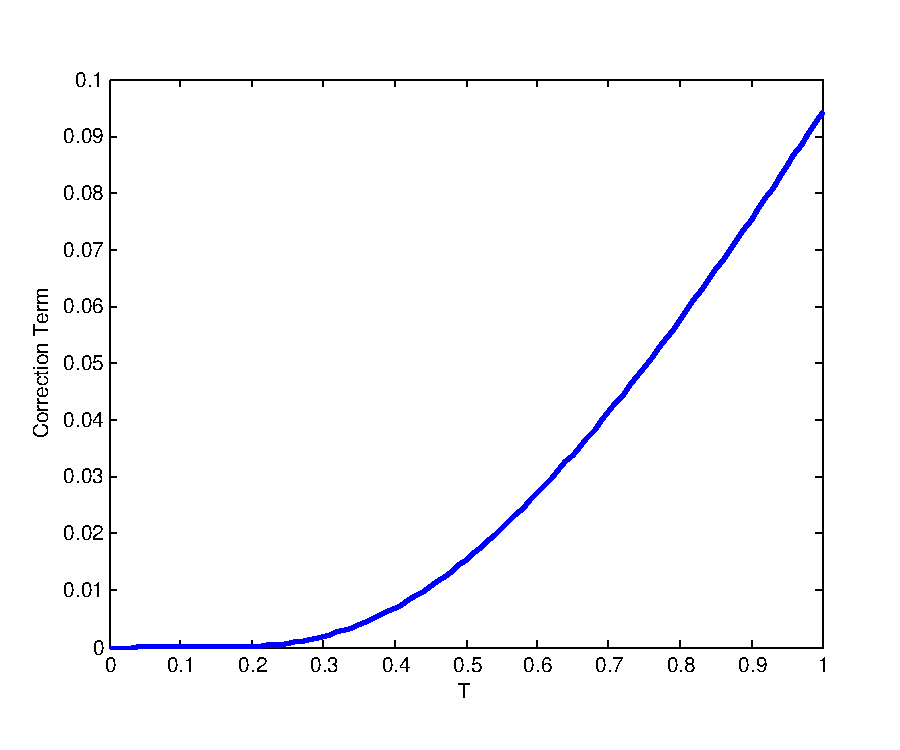
\includegraphics[width=3.5in]{03.integrals/c_electron.pdf}}
\caption{Correction term, the integral in Eq. (\ref{eq:delta_heat_electron}).}
\label{fig:heat_electron}
\end{figure}

\newpage
\noindent
\section*{Problems}
\addcontentsline{toc}{section}{\protect\numberline{}Problems}

\begin{enumerate}[labelwidth=0.5cm,labelindent=0cm,leftmargin=*,label=\bfseries \thechapter.\arabic*,align=left]
%
\item Integrate $x \cos x$ from $x=0$ to $x=\pi$ using Trapezoidal and Simpson rules.  Compare the results with the exact solution $\int x \cos x\, \md x = \cos x + x \sin x$.
%
\item Plot the molar heat capacity of copper ($\theta_D=309\, K$) from $T=0\, K$ to $T=1083\, K$ using the Debye theory shown in Section \ref{sec:debye}. 
%
\item Write a code to produce Fig. \ref{fig:heat_electron}.
\end{enumerate}

\newpage
\section*{Appendix}
\addcontentsline{toc}{section}{\protect\numberline{}Appendix}

\appendix{Expansion of Integral with $h$}\label{ap:int_expand}

\medskip\noindent
Consider the integral as a function of $h$ as
\begin{equation}
F(h) = \int_{x_n}^{x_n+h} f(x) \dd{x}
\end{equation}
and expand it in a McLaughlin series
\begin{equation}\label{eq:int_McLaughlin}
F(h) = F(0) + F'(0) h + \frac{1}{2} F''(0) h^2 + \frac{1}{3!} F^{(3)}(0) h^3 + \frac{1}{4!} F^{(4)}(0) h^4 + o(h^5)\, .
\end{equation}
Obviously, $F(0)=0$. The first derivative of $F(x)$ can be computed as
\begin{equation}
F'(h) = \dv{h} \int_{x_n}^{x_n+h} f(x) \dd{x} =  \dv{z} \int_{x_n}^{z} f(x) \dd{x} = f(z)=f(x_n+h)
\end{equation}
where $z=x_n+h$.  Higher order derivatives are now simply $F^{(k)}(h)=f^{(k-1)}(x_n+h)$. Substituting these results into the expansion (\ref{eq:int_McLaughlin}), we obtain Eq, (\ref{eq:int+expand}).

\bigskip

\appendix{Justification of Gaussian Quadrature}
\label{app:gauss-quad}

To be written.


\newpage
\appendix{Gaussian Quadrature: Weights and Abscissas}

\renewcommand{\arraystretch}{1.5}

\begin{table}[h]
\caption{Weights and Abscissas for Gaussian-Laguerre quadrature}
\tiny
\begin{center}
\begin{tabular}{|c|ll|}
\hline
\multicolumn{1}{|c|}{$N$}&\multicolumn{1}{c}{$x$}&\multicolumn{1}{c|}{$w$}\\
\hline
 2
  &5.8578 6437 6269 0495$\times 10^{-1}$ &8.5355 3390 5932 7376$\times 10^{-1}$\\
  &3.4142 1356 2373 0950                 &1.4644 6609 4067 2624$\times 10^{-1}$\\
\hline
4
  &3.2254 7689 6193 9231$\times 10^{-1}$ &6.0315 4104 3416 3360$\times 10^{-1}$\\
  &1.7457 6110 1158 3466 &3.5741 8692 4377 9969$\times 10^{-1}$\\
  &4.5366 2029 6921 1280 &3.8887 9085 1500 5384$\times 10^{-2}$\\
  &9.3950 7091 2301 1331 &5.3929 4705 5613 2745$\times 10^{-4}$\\
\hline
6
  &2.2284 6604 1792 6069$\times 10^{-1}$ &4.5896 4673 9499 6359$\times 10^{-1}$\\
  &1.1889 3210 1672 6230                 &4.1700 0830 7721 2099$\times 10^{-1}$\\
  &2.9927 3632 6059 3141                 &1.1337 3382 0740 4498$\times 10^{-1}$\\
  &5.7751 4356 9104 5105                 &1.0399 1974 5314 9075$\times 10^{-2}$\\
  &9.8374 6741 8382 5899                 &2.6101 7202 8149 3206$\times 10^{-4}$\\
  &1.5982 8739 8060 1702$\times 10^{+1}$ &8.9854 7906 4296 2124$\times 10^{-7}$\\
\hline
8
  &1.7027 9632 3051 0100$\times 10^{-1}$ &3.6918 8589 3416 3753$\times 10^{-1}$\\
  &9.0370 1776 7993 7991$\times 10^{-1}$ &4.1878 6780 8143 4296$\times 10^{-1}$\\
  &2.2510 8662 9866 1307                 &1.7579 4986 6371 7181$\times 10^{-1}$\\
  &4.2667 0017 0287 6588                 &3.3343 4922 6121 5652$\times 10^{-2}$\\
  &7.0459 0540 2393 4657                 &2.7945 3623 5225 6725$\times 10^{-3}$\\
  &1.0758 5160 1018 0995$\times 10^{+1}$ &9.0765 0877 3358 2131$\times 10^{-5}$\\
  &1.5740 6786 4127 8005$\times 10^{+1}$ &8.4857 4671 6272 5315$\times 10^{-7}$\\
  &2.2863 1317 3688 9264$\times 10^{+1}$ &1.0480 0117 4871 5104$\times 10^{-9}$\\
\hline
\end{tabular}\label{tab:Gaussian-Laguerre}
\end{center}
\end{table}


\newpage
\begin{table}[h]
\caption{Weights and Abscissas for Gaussian-Hermite Quadrature.
Abscissas are symmetric with respect to $x=0$.  Therefore, for every positive abscissa $x$ there is negative one $-x$. Only non-negative abscissas are shown.}
\footnotesize
\begin{center}
\begin{tabular}{|c|ll|}
\hline
\multicolumn{1}{|c|}{$N$} & \multicolumn{1}{c}{$\pm x$} & \multicolumn{1}{c|}{$w$}\\
\hline
2 
  & 0.7071067811 & 0.8862269254\\
\hline
3 
  & 0            & 1.1816359006\\
  & 1.2247448713 & 0.2954089751\\
\hline
4 
  & 0.5246476232 & 0.8049140900\\
  & 1.6506801238 & 0.0813128354\\
\hline
5 & 0            & 0.9453087204\\
  & 0.9585724646 & 0.3936193231\\
  & 2.0201828704 & 0.0199532420\\
\hline
6 & 0.4360774119 & 0.7246295952\\
  & 1.3358490740 & 0.1570673203\\
  & 2.3506049736 & 0.0045300099\\
\hline
7 & 0            & 0.8102646175\\
  & 0.8162878828 & 0.4256072526\\
  & 1.6735516287 & 0.0545155828\\
  & 2.6519613568 & 0.0009717812\\
\hline
8 & 0.3811869902 & 0.6611470125\\
  & 1.1571937124 & 0.2078023258\\
  & 1.9816567566 & 0.0170779830\\
  & 2.9306374202 & 0.0001996040\\
  \hline
\end{tabular}\label{tab:Gaussian-Hermite}
\end{center}
\end{table}

\vfill
\newpage

\begin{table}[h]
\center
\caption{Weights and Abscissas for Gaussian-Legendre Quadrature. Abscissas are symmetric with respect to $x=0$.  Therefore, for every positive abscissa $x$ there is negative one $-x$. Only non-negative abscissas are shown.}
\footnotesize
\begin{center}
\begin{tabular}{|c|ll|}
\hline
\multicolumn{1}{|c|}{$N$}&\multicolumn{1}{c}{$\pm x$}&\multicolumn{1}{c|}{$w$}\\
\hline
2 
  & 0.5773502692 & 1            \\
\hline
3 
  & 0            & 0.8888888889\\
  & 0.7745966692 & 0.5555555556\\
\hline
4 
  & 0.3399810436 & 0.6521451549\\
  & 0.8611363116 & 0.3478548451\\ 
\hline
5 
  & 0            & 0.5688888889\\
  & 0.5384693101 & 0.4786286705\\
  & 0.9061798459 & 0.2369268851\\
\hline
6
  & 0.2386191861 & 0.4679139346\\
  & 0.6612093865 & 0.3607615730\\
  & 0.9324695142 & 0.1713244924\\
\hline
7 
  & 0            & 0.4179591837\\
  & 0.4058451514 & 0.3818300505\\
  & 0.7415311856 & 0.2797053915\\
  & 0.9491079123 & 0.1294849662\\
\hline
8 & 0.1834346425 & 0.3626837834\\
  & 0.5255324099 & 0.3137066459\\
  & 0.7966664774 & 0.2223810345\\
  & 0.9602898565 & 0.1012285363\\
\hline
\end{tabular}\label{tab:Gaussian-Legendre}
\end{center}
\end{table}



\newpage
\section*{MATLAB Source Codes}
\addcontentsline{toc}{section}{\protect\numberline{}MATLAB Source Codes}

\bigskip\noindent
\program
\label{matlab:integrals}
\footnotesize
\begin{verbatim}
%**************************************************************************
%*     Example  3.1                                                       *
%*     filename: ch03pr01.m                                               *
%*     program listing number: 3.1                                        *
%*                                                                        *
%*  This program integrate sin(x) from x=0 to x=pi using rectangular,     *
%*  trapezoidal and simpson methods.  Absolute errors are plotted.        *
%*                                                                        *
%*     Programed by Ryoichi Kawai for Computational Physics Course.       *
%*     Last modification:  01/14/2019.                                    *
%**************************************************************************

clear all;

% Set the lower and upper bound of the integration
a=0;
b=pi/2;

% Header of the output
display('    Absolute error in various numrical integration')
fprintf(' %3s %21s %24s %24s\n','N','Rectangular','Trapezoidal','Simpson');

% loop over different N
for k=1:10
    N=2^k;
    h(k)=(b-a)/N;
    
    % evaluate the variable and function
    for i=0:N
         x(i+1)=a+i*h(k);
         f(i+1)=sin(x(i+1));
    end
    
    % Rectangular rule
    rect=sum(f(1:N))*h(k);
    
    % Trapezoidal rule
    trap=sum(f(2:N))*h(k) + (f(1)+f(N+1))*h(k)/2;
    
    % Simpson rule
    simp=(2*sum(f(1:2:N-1))+4*sum(f(2:2:N))-f(1)+f(N+1))*h(k)/3;
    
    % Evaluation of errors (the exat answer is 1)
    err_rect(k)=abs(1-rect);
    err_trap(k)=abs(1-trap);
    err_simp(k)=abs(1-simp);
    
    %print out the results
    fprintf('   %5d %24.16e %24.16e %24.16e \n',...
        N,err_rect(k),err_trap(k),err_simp(k));
end

% Order of the errors
h2=h.^2;
h3=h.^3;
h4=h.^4;

% Plot the results
subplot(1,1,1)
p=loglog(h,err_rect,'d',h,err_trap,'o',h,err_simp,'s',...
    h,h,'--',h,h2,'--',h,h4,'--');

% Format the plot
title('Absolute errors in the various integration methods');
xlabel('h');
ylabel('absolute error');
set(p(1),'Color','green');
set(p(2),'Color','blue');
set(p(3),'Color','red');
set(p(4),'Color','green','LineWidth',2);
set(p(5),'Color','blue','LineWidth',2);
set(p(6),'Color','red','LineWidth',2);
legend(p,{'rectangular','trapezoidal','simpson','h','h^2','h^4'});
legend(p,'Location','SouthEast');
\end{verbatim}
\normalsize

\ruleend

\bigskip
\noindent
\program
\label{matlab:improper_int}
\footnotesize
\begin{verbatim}
%*********************************************************************
%*     Example 3.3                                                   *
%*     filename: ch03pr02.m                                          *
%*     program listing number: 3.2                                   *
%*                                                                   *
%*     This program integrates 1/(sqrt(x)*(1+x)) from x=0 to x=1     *
%*     by removing singularity at x=0.  Trapezoidal rule is used     *
%*     for the proper part of integral.                              *
%*                                                                   *
%*     Programed by Ryoichi Kawai for Computational Physics Course   *
%*     Revised on 01/07/2014.                                        *
%*********************************************************************

clear all;
a = 1.0;  % upper bound
N = 100;  % number of segments
h = a/N;  % width of segments

% integration of sqrt(x)/(1+x) with trapezoidal rule
S = sqrt(a)/(1+a)/2;  %bundary value devided by 2
for i=1:N-1
    x = i*h;
    f = sqrt(x)/(1+x);
    S = S +f;
end
proper = S*h;  % integral of proper part

singular = 2*sqrt(a);  % singular part

total = singular - proper; 
exact = pi - 2*atan(1/sqrt(a));

fprintf('Numerical = %18.12e\n',total);
fprintf('    Exact = %18.12e\n',exact);
\end{verbatim}
\normalsize

\ruleend

\newpage
\bigskip
\noindent
\program
\label{matlab:gauss-lagurre}
\footnotesize
\begin{verbatim}
%**************************************************************************
%*     Example  3.4                                                       *
%*     filename: ch03pr03.m                                               *
%*     program listing number: 3.3                                        *
%*                                                                        *
%*  This program numerically integrates x^3*exp(x)/(exp(x)-1) from        *
%*  x=0 to infinity using 8-point Gaussian Laguerre Quadrature.           *
%*                                                                        *
%*     Programed by Ryoichi Kawai for Computational Physics Course.       *
%*     Last modification:  01/06/2014.                                    *
%**************************************************************************
clear all;

N=8;

x=[1.7027963230510100e-1, 9.0370177679937991e-1,...
   2.2510866298661307,    4.2667001702876588,   ...
   7.0459054023934657,    1.0758516010180995e+1,...
   1.5740678641278005e+1, 2.2863131736889264e+1];
w=[3.6918858934163753e-1, 4.1878678081434296e-1,...
   1.7579498663717181e-1, 3.3343492261215652e-2,...
   2.7945362352256725e-3, 9.0765087733582131e-5,...
   8.4857467162725315e-7, 1.0480011748715104e-9];

for i=1:N
    f(i)=x(i)^3*exp(x(i))/(exp(x(i))-1);
end

Gauss=sum(w.*f);
Exact=pi^4/15;
fprintf('%i points Gaussian Laguerre Quadrature\n',N);
fprintf(' Exact=%18.12e\n Gauss=%18.12e\n Error=%18.12e\n',...
Exact,Gauss,abs(Exact-Gauss));
\end{verbatim}
\normalsize

\bigskip
\noindent
\section*{Examples in Python}
\addcontentsline{toc}{section}{\protect\numberline{}Examples in Python}

\bigskip
\setcounter{exampnum}{1}

\noindent
\begin{example}[Adaptive Quadrature]

A Python package called SciPy has  built-in function \texttt{quad(func,xmin,xmax)} which uses adaptive quadrature with a default error tolerance.
\begin{center}
\begin{minipage}{0.95\textwidth}
\small
\begin{Verbatim}[frame=single]
>>> import numpy as np
>>> import scipy.integrate as spint
>>> y=spint.quad(lambda x: (4.0*x-x**2)*np.exp(-2.0*x),0.0,5.0)
>>> print(y)
\end{Verbatim}
\normalsize
\end{minipage}
\end{center}

\noindent
You can create a function and pass it to a subprogram by 'lambda x:  (4.0*x-x**2)*np.exp(-2.0*x)'.  This is a unique capability of Python.
\end{example}

\newpage
\normalsize
\noindent
\section*{Python Source Codes}
\addcontentsline{toc}{section}{\protect\numberline{}Python Source Codes}
\setcounter{program}{0}

\bigskip\noindent
\program
\label{python:integrals}
\footnotesize
\begin{verbatim}
# -*- coding: utf-8 -*-
"""
%**************************************************************************
%*  Example  3.1                                                          *
%*  filename: ch03pr01.py                                                 *
%*  program listing number: 3.1                                           *
%*                                                                        *
%*  This program integrate sin(x) from x=0 to x=pi using rectangular,     *
%*  trapezoidal and simpson methods.  Absolute errors are plotted.        *
%*                                                                        *
%*     Programed by Ryoichi Kawai for Computational Physics Course.       *
%*     Last modification:  01/14/2019.                                    *
%**************************************************************************
"""

import numpy as np
import scipy.integrate as integrate
import matplotlib.pyplot as plt

opt=input("Use SciPy [y/n] ")
if opt=='y':
print("SciPy integrate will be used.\n")
else:
print("SciPy will not be used.\n")

# Set the lower and upper bound of the integration
a=0.
b=np.pi/2.
# Header of the output
print("{0:^75}".format('Absolute error in various numrical integration'))
print("{0:^6} {1:^23} {2:^24} {3:^24} \n"
.format('N','Rectangular','Trapezoidal','Simpson'))

kmax=10
h=np.zeros(kmax+1)
err_rect=np.zeros(kmax+1)
err_trap=np.zeros(kmax+1)
err_simp=np.zeros(kmax+1)

for k in range(0,kmax):
N=2**(k+1)
h[k]=(b-a)/N

x = a + np.linspace(a,b,N+1)
f = np.sin(x)

rect=f[0:N].sum()*h[k]

if opt=='y':
trap=integrate.trapz(f,x)
simp=integrate.simps(f,x)
else:      
trap=f[1:N].sum()*h[k]+(f[0]+f[N])*h[k]/2.    
simp=(2.0*f[0:N-1:2].sum()+4.0*f[1:N:2].sum()-f[0]+f[N])*h[k]/3. 

err_rect[k]=abs(1.-rect)
err_trap[k]=abs(1.-trap)
err_simp[k]=abs(1.-simp)

print("{0:5d} {1:24.16e} {2:24.16e} {3:24.16e}"
.format(N,err_rect[k],err_trap[k],err_simp[k]))

del x
del f

# Plot data
h2=h**2
h3=h**3
h4=h**4

plt.ioff()
plt.figure(figsize=(6,5))
plt.loglog(h,err_rect, 'og', label='rectangular')
plt.loglog(h,err_trap, 'ob', label='trapezoidal')
plt.loglog(h,err_simp, 'or', label='simpson')
plt.loglog(h,h,'--g',label='$h$')
plt.loglog(h,h2,'--b',label='$h^2$')
plt.loglog(h,h4,'--r',label='$h^4$')
plt.legend(loc=4)
plt.xlabel('h')
plt.ylabel('Integral')
plt.show()
\end{verbatim}

\normalsize

\ruleend

\bigskip
\noindent
\program
\label{python:improper_int}
\footnotesize
\begin{verbatim}
#!/usr/bin/env python3
"""
%**************************************************************************
%*  Example  3.3                                                          *
%*  filename: ch03pr02.py                                                 *
%*  program listing number: 3.2                                           *
%*                                                                        *
%*  This program integrates 1/(sqrt(x)*(1+x)) from x=0 to x=1             *
%*  by removing singularity at x=0. Trapezoidal rule is used              *
%*  for the proper part of integral.                                      *
%*                                                                        *
%*     Programed by Ryoichi Kawai for Computational Physics Course.       *
%*     Last modification:  01/11/2017.                                    *
%**************************************************************************
"""
import numpy as np

a = 1.0 # upper bound
N = 100 # number of segments
h = a/N # width of segments
# integration of sqrt(x)/(1+x) with trapezoidal rule
S = np.sqrt(a)/(1.0+a)/2.0; # bundary value devided by 2
for i in range(1,N):
    x = i*h
    f = np.sqrt(x)/(1+x)
    S = S +f

proper = S*h # integral of proper part
singular = 2*np.sqrt(a)
# singular part
total = singular - proper
exact = np.pi - 2*np.arctan(1/np.sqrt(a))
print("Numerical = {0:18.12e}".format(total))
print("    Exact = {0:18.12e}".format(exact))
\end{verbatim}

\normalsize

\ruleend

\bigskip
\noindent
\program
\label{python:gauss-lagurre}
\footnotesize
\begin{verbatim}
#!/usr/bin/env python3
# -*- coding: utf-8 -*-
"""
%**************************************************************************
%*  Example  3.4                                                          *
%*  filename: ch03pr03.py                                                 *
%*  program listing number: 3.3                                           *
%*                                                                        *
%*  This program numerically integrates x^3*exp(x)/(exp(x)-1) from        *
%*  x=0 to infinity using 8-point Gaussian Laguerre Quadrature.           *
%*                                                                        *
%*     Programed by Ryoichi Kawai for Computational Physics Course.       *
%*     Last modification:  01/12/2019.                                    *
%**************************************************************************
"""
import numpy as np

def f(x):
    return x**3*np.exp(x)/(np.exp(x)-1.)

if __name__ == "__main__":    
    N=8
# evaluation points and weights for 8 point Gaussian quadrature
    x=np.array([1.7027963230510100e-1, 9.0370177679937991e-1,
                2.2510866298661307,    4.2667001702876588,
                7.0459054023934657,    1.0758516010180995e+1,
                1.5740678641278005e+1, 2.2863131736889264e+1])

    w=np.array([3.6918858934163753e-1, 4.1878678081434296e-1,
                1.7579498663717181e-1, 3.3343492261215652e-2,
                2.7945362352256725e-3, 9.0765087733582131e-5,
                8.4857467162725315e-7, 1.0480011748715104e-9])

    gauss=(w*f(x)).sum()  #Gaussian quadrature
    exact=np.pi**4/15.
    print("{0:3d} point Gaussian Laguerre Quadrature".format(N))
    print("  Exact={0:18.12e}\n Gauss={1:18.12e}\n  Error={2:18.12e}"
          .format(exact,  gauss, abs(exact-gauss)))
\end{verbatim}
\normalsize

\newpage


\bibliographystyle{unsrt}
\bibliography{compphys}

\vfill
